% WASP Software Engineering Course - Assignment Template (2026)
% Overleaf-ready LaTeX template
% Replace all TODO text with your own analysis before submission.

\documentclass[11pt,a4paper]{article}

% --- Page layout and typography ---
\usepackage[a4paper,margin=3cm]{geometry}
\usepackage{newtxtext,newtxmath} % Times-like font, Overleaf compatible
\usepackage[T1]{fontenc}
\usepackage[utf8]{inputenc}
\usepackage{microtype}
\usepackage{setspace}
\usepackage{parskip}
\usepackage{enumitem}
\usepackage{graphicx}
\usepackage{booktabs}
\usepackage{xcolor}
\usepackage{hyperref}

\usepackage{tikz}
\usepackage{graphicx}
\usetikzlibrary{chains,shapes.multipart}
\usetikzlibrary{shapes,calc}
\usetikzlibrary{automata,positioning}
\usetikzlibrary{positioning, shapes, arrows, calc}
\tikzstyle{block} = [draw, rectangle, line width=0.7mm]

\usepackage[nameinlink,noabbrev]{cleveref}
\usepackage{csquotes}

% --- References ---
% Recommended Overleaf setup: create a references.bib file and add your sources there.
\usepackage[
    backend=biber,
    style=numeric
]{biblatex}

\addbibresource{references.bib}


% --- Hyperlink setup ---
\hypersetup{
    colorlinks=true,
    linkcolor=black,
    citecolor=blue!60!black,
    urlcolor=blue!60!black,
    pdftitle={WASP Software Engineering Assignment 2026},
    pdfauthor={Your Name}
}

% --- Small helper commands for drafting ---
\newcommand{\todo}[1]{\textcolor{red!70!black}{\textbf{TODO:} #1}}
\newcommand{\guidance}[1]{%
    \begin{quote}\small\color{gray!75!black}\emph{#1}\end{quote}%
}

\title{Software Engineering for AI/AS: Reflections from My Research}
\author{fethi bencherki\\
WASP Software Engineering Course, Module 2026\\
\texttt{fethi.bencherki@control.lth.se}}
\date{September 1, 2026}

\begin{document}
\maketitle



\section{Introduction}

At a high level, my research concerns the \emph{online optimal control of dynamical systems whose dynamics are not completely known a priori}. In a classical control problem, a mathematical model describing how the system evolves is assumed to be available before the controller is designed. In many real-world settings, however, such a model is either uncertain or only partially known. The controller must therefore learn the physics of the system while simultaneously making decisions that regulate its behavior. This creates a fundamental exploration--exploitation trade-off: some control actions are useful because they reveal information about the unknown system, whereas others are chosen primarily because they improve the immediate control objective.

Controllers that explicitly account for these two objectives are commonly referred to as \emph{dual controllers}. Their actions have a dual purpose:
\begin{enumerate}
\item[\it{(1)}] \textbf{Probing}: selecting actions that provide information about the unknown system dynamics; 
\item[\it{(2)}] \textbf{Exploiting}: using the acquired knowledge to make increasingly effective control decisions.
\end{enumerate}
This perspective is closely related to the learning and decision-making principle underlying reinforcement learning (RL). However, an important emphasis of my research is on developing methods for which properties such as stability, robustness, and control performance can be characterized through formal mathematical guarantees. Such guarantees support the safe and trustworthy operation of the physical system being controlled, especially in safety critical applications.

Within this broader framework, I focus on \emph{positive linear systems}. These are dynamical systems whose relevant physical quantities remain non-negative, a structure that naturally appears in applications involving quantities such as populations, concentrations, inventories, traffic flows, or resource levels. Positivity provides additional mathematical structure that can be exploited to develop scalable analysis and control methods. This is particularly useful when moving from individual systems to large-scale interconnected systems and networks, where conventional control and optimization methods can become computationally prohibitive. At the same time, increasing system size and complexity makes accurate modeling more difficult, as uncertain parameters, external disturbances, and unmodeled dynamics become harder to capture. The controller must therefore remain effective despite these modeling imperfections, as illustrated in Fig.~\ref{fig:prob}.


From a software engineering perspective, reliable operation extends beyond the controller itself. In practice, the controller is part of a larger cyber-physical system that integrates sensing, online system identification, optimization, and actuation in a continuous closed loop. Reliability therefore depends not only on the mathematical guarantees of the control algorithm, but also on how these components are implemented, integrated, tested, and monitored. This is where software engineering for AI/AS becomes particularly relevant to my research.

\begin{figure}
    \centering
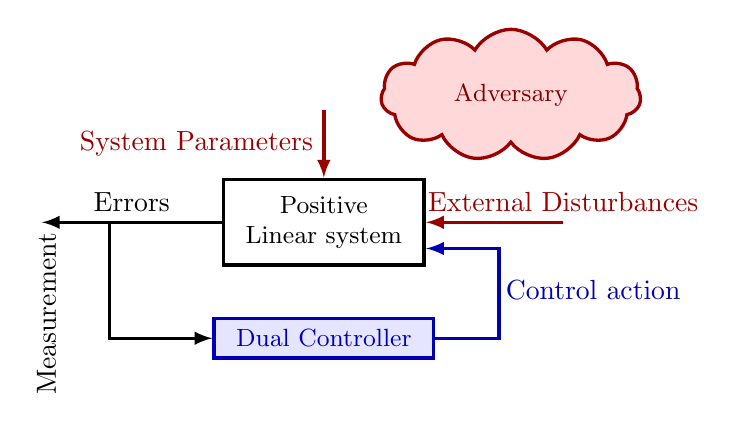
\begin{tikzpicture}[
    >=latex,scale=0.95,
    block/.style={
        draw,
        line width=1.4pt,
        rectangle,
        inner xsep=8pt,
        inner ysep=6pt,
        align=center,
        font=\small
    },
    controller/.style={
        draw=blue!70!black,
        line width=1.2pt,
        rectangle,
        inner xsep=8pt,
        inner ysep=4pt,
        align=center,
        font=\small,
        fill=blue!10
    },
    adversary/.style={
        draw=red!60!black,
        line width=1.2pt,
        fill=red!15,
        cloud,
        cloud puffs=11,
        cloud puff arc=120,
        cloud ignores aspect,
        inner xsep=12pt,
        inner ysep=8pt,
        align=center,
        font=\small,
        text=red!50!black
    },
    redarrow/.style={->, line width=1.2pt, red!60!black},
    bluearrow/.style={->, line width=1.2pt, blue!70!black},
    blackarrow/.style={->, line width=1.2pt}
]

% Nodes
\node[block] (plant) at (0,0) {Positive\\Linear system};
\node[controller, text=blue!70!black] (ctrl) at (0,-1.55)
{Dual Controller};
\node[adversary] (adv) at (2.5,1.7) {Adversary};

% Output arrow
\draw[blackarrow] (plant.west) -- ++(-2.4,0)
    node[midway, above] {Errors};

% Measurement path
% \draw[blackarrow] ($(plant.west)+(-1.5,0)$) |- (ctrl.west)
%     node[pos=0.35, left] {State Measurement};
\draw[blackarrow] ($(plant.west)+(-1.5,0)$) |- (ctrl.west)
    node[pos=0, left,xshift=-8mm, rotate=90] {Measurement}; %State 
% Control path
\draw[bluearrow] (ctrl.east) -- ++(0.85,0) |- ($(plant.east)+(0,-0.35)$);
\node[blue!70!black] at (3.6,-0.9) {Control action};

% Disturbance arrow
\draw[redarrow] (3.2,0) -- (plant.east)
    node[pos=0, above] {External Disturbances};

% Parameters arrow
\draw[redarrow] (0,1.5) -- (plant.north)
    node[midway, left] {System Parameters};

\end{tikzpicture}
\caption{Dual control of a positive linear system with uncertain dynamics and external disturbances. The controller simultaneously learns about the unknown system through its actions and exploits the acquired information to improve control performance.}
    \label{fig:prob}
\end{figure}



\section{Lecture Principles}


\subsection{Principle 1: Iterate Rather Than Design Everything Upfront}

In Lecture 1, one software engineering principle is that ``Big X upfront rarely pays off,'' because there is often not enough knowledge early in development; instead, the system should be developed iteratively. This is particularly relevant for AI-intensive systems, where requirements, data characteristics, and model behavior may only become clear through experimentation and use.

This principle aligns closely with my research on online control of initially unknown systems. Since the controller does not know the true dynamics in advance, it must progressively improve its model while interacting with the system. From a software engineering perspective, this suggests structuring the implementation so that system identification, controller design, and evaluation can be refined incrementally rather than assuming that a complete and accurate model is available from the beginning. It also motivates modular software components that allow the estimation and control algorithms to be updated independently as new knowledge becomes available to the controller.

\subsection{Principle 2: Test Early, Test Often, Test Throughout, Test Automatically}

Another explicit principle is to ``test early, test often, test throughout, test automatically.'' For AI-intensive systems, testing only a final implementation or a few nominal examples gives limited evidence about how the complete system behaves under changing or uncertain conditions.

This is directly relevant to robustness evaluation in my research. A controller should not only be tested on its nominal model, but also across uncertain parameters, disturbances, initial conditions, measurement noise, and modeling errors. Formal analysis and testing therefore complement each other: mathematical results establish guarantees under stated assumptions, while automated simulations check whether the implemented controller behaves consistently with those guarantees. In my project, this could be realized through automated scenarios that monitor stability, control cost, constraint violations, estimation error, and computational efficiency. This aspect is especially important in critical applications, where downtime and safety are critical concerns.




\section{Guest Lecture Principles}



\subsection{Guest-Lecture Principle 1: Changing Quality Priorities in AI Systems}


In Julian Frattini's guest lecture \emph{Requirements Engineering for Artificial Intelligence-based Systems}, an important observation is that introducing AI can change which software qualities matter most. Compared with traditional software, qualities such as accuracy, fairness, maintainability, and retrainability may become more important, while entirely new quality concerns can also emerge. This means that evaluating an AI-intensive system requires considering several quality attributes rather than focusing only on the predictive or algorithmic performance of its AI component.

This perspective is relevant to my research because controller performance is only one aspect of the quality of an online control system. Robustness to uncertainty, computational efficiency, scalability to large networks, and the ability to update the controller as new information becomes available are also important. These qualities can also conflict; for example, achieving stronger robustness guarantees may require more conservative control actions or additional computation. The lecture therefore highlights the need to evaluate my methods across several system level criteria and to make the associated trade-offs explicit rather than judging a controller only by its nominal control cost.
%(slide 7)

\subsection{Guest Lecture Principle 2: AI-Mediated Work Changes Workflows and Accountability}


In Per Lenberg's guest lecture on \emph{Behavioral Software Engineering}, the ``semi-executable stack'' illustrates how AI-mediated software engineering changes not only code generation but also workflows and responsibilities. Traditional human workflows may become agentic or human--AI workflows, while reviews and quality assurance activities may increasingly involve automated evaluation. The lecture also highlights that roles, decision rights, and accountability can change as AI takes a larger role in decision making.

This principle becomes relevant when considering the deployment of an adaptive controller. Even if the controller has formal guarantees, responsibility for monitoring its operation and deciding when intervention is required still has to be clearly assigned. As the controller becomes more autonomous and adapts from observations, engineers or operators must understand its operating limits and how to respond when those limits are exceeded. A key challenge is therefore to increase autonomy without making responsibility and accountability for the resulting decisions unclear.

\section{Data Scientists, Software Engineers, and AI Engineers}
\label{sec:roles}

\subsection{From Model Development to System Engineering}

The CMU \emph{Machine Learning in Production} book in~\cite{kastner2025machine} describes data scientists as being mainly concerned with data, models, and experimentation, whereas software engineers are more concerned with the complete system and its lifecycle, including requirements, testing, deployment, scalability, and maintenance. I think this distinction is useful, although in practice it is not always so clear. Once a learned model becomes part of a working system, decisions made during model development can have consequences for the software around it.

Chapter 2 extends this distinction by arguing that a good ML model does not necessarily imply a good overall system. The model is only one component, and its usefulness depends on how it interacts with other software, users, and the environment. I see the same issue in my research. Developing an online controller involves learning and algorithm design, but an implementation also has to satisfy computational and numerical constraints while interacting with a physical system in real time. Measurements are used to update knowledge about the dynamics, this knowledge influences the control action, and the action changes the system from which future measurements are obtained. Stability, robustness, and safety therefore have to be considered for the complete closed loop rather than for the learning algorithm in isolation.

\subsection{The Evolving Roles of Data Scientists and Software Engineers}

I think data scientists and software engineers will remain different specializations, but the overlap between them will continue to grow. Data scientists working with deployed models need some understanding of testing, deployment, and system constraints, while software engineers working with AI components need to understand model uncertainty, data quality, and evaluation. This does not mean that everyone needs the same expertise, but both groups need enough understanding of each other's work to develop and maintain the same system effectively.

\subsection{The Role of AI Engineering}

I see AI Engineering as sitting between these roles rather than simply replacing either of them. It includes parts of MLOps and model engineering, but its scope is broader when AI is a central component of a larger software system. To me, AI Engineering is therefore mainly concerned with turning AI or learning components into reliable engineered systems. The important question is not only whether the model or algorithm performs well, but whether the complete system remains reliable when it interacts with conventional software, users, data, and its environment.

\subsection{Foundation Models and Changing Role Boundaries}

Foundation models make these boundaries even less clear. Building an AI application no longer necessarily means training a model; it can instead involve selecting an existing model and building prompts, RAG pipelines, evaluations, or agentic workflows around it. AI coding assistants also allow software engineers to work more directly with AI while helping data scientists produce and maintain software. I therefore expect the roles to overlap further. At the same time, as AI components are given more autonomy and access to external tools, engineering concerns such as testing, monitoring, failure handling, safety, and accountability become more important rather than less.





\section{Paper Analysis}
\label{sec:paper-analysis}

\subsection{Paper 1: Jie JW Wu -- \emph{An Exploratory Study of V-Model in Building ML-Enabled Software: A Systems Engineering Perspective} in~\cite{wu2024exploratory}}

The paper looks at a problem that occurs when moving from an ML model developed experimentally to an actual software system. In particular, ML development and software development are often carried out by people with different backgrounds and workflows. Based on interviews with practitioners, the paper investigates whether the V-Model from systems engineering can provide more structure to this process. The basic idea I take from the paper is that development decisions should have corresponding verification and validation activities, instead of treating testing as something that comes only after the model or algorithm is finished. From an SE perspective, this is important because the quality of an ML component alone does not guarantee the reliability of the system in which it is integrated.

This made me think about the gap between how I currently view my research and how the resulting controller would actually be used. Most of my work is concerned with the controller itself: given assumptions about the system and its uncertainty, I want to establish stability, robustness, or performance guarantees. In practice, however, the controller would be deployed inside a much larger system. Measurements have to be collected and processed, parameters have to be estimated, an optimization problem has to be solved, and the resulting control input has to be sent to the physical system. A proof about the control law does not automatically guarantee that this whole chain works correctly.

For example, consider using my controller in a large traffic, energy, or resource network, where online learning and adaptation are core parts of the system's functionality. My research would provide the online identification and control components, while the complete project would also require sensors, communication, optimization software, actuator interfaces, and monitoring. The V-Model could be useful here because different assumptions and requirements could be connected to corresponding verification activities. Mathematical analysis could verify stability and robustness, software tests could check the numerical implementation, and system level simulations could evaluate the complete closed-loop system during operation.

One change I could make in my own work is to create a clearer link between theoretical guarantees and their practical implementation. For example, assumptions on uncertainty bounds, disturbance levels, or computation time could be translated into conditions that can be tested or monitored during operation. Similarly, documenting component interfaces and potential failure modes would make it clearer how the controller can be integrated into a larger system. Applying the complete V-Model may be excessive for a primarily theoretical research project, but its underlying idea of connecting design decisions and assumptions with corresponding verification activities is valuable. This could help bridge the gap between proving that a controller works mathematically and demonstrating that its implementation behaves reliably in a real system.


\subsection{Paper 2: Giamattei et al. -- \emph{Reinforcement Learning for Online Testing of Autonomous Driving Systems: a Replication and Extension Study} in \cite{giamattei2025reinforcement}}

The paper is interesting to me because it uses reinforcement learning in an unusual way. The RL agent does not control the autonomous vehicle; instead, it acts as a tester and searches for environmental conditions that cause the autonomous driving system to violate functional or safety requirements. Another important aspect is that the authors first attempt to replicate an earlier result but do not obtain the previously reported advantage of RL over random testing. They then reformulate the problem and use a deep RL approach better suited to the state space, after which RL performs better. From an SE perspective, this demonstrates both the potential of automated testing for complex AI systems and the importance of careful experimental design, reproducibility, and appropriate testing baselines.

There is a direct connection to my research. In dual control, the controller interacts with a dynamical system and uses the resulting observations to decide what to do next. The testing agent in this paper also learns through sequential interaction, but its objective is almost the opposite. My controller tries to maintain good performance despite uncertainty, while the testing agent actively searches for situations where the system performs poorly. This is also similar to the adversarial side of the problem in Fig.~\ref{fig:prob}, where disturbances and uncertain parameters work against the controller.

I could imagine combining these ideas in a larger AI-intensive control project, for example a large autonomous traffic, energy, or resource network. My adaptive controller would provide the online learning and decision making functionality of the system. During development, a separate RL testing agent could interact with a simulator and vary disturbances, uncertain parameters, or initial conditions. Instead of generating test cases randomly, the agent would learn which combinations are most likely to produce constraint violations, high control costs, or behavior close to instability. In this setting, my controller would be the system under test, while RL would provide an adaptive stress testing mechanism.

This approach would complement, rather than replace, the formal robustness guarantees that are central to my research. While repeated simulations cannot provide the same guarantees as a mathematical proof, an RL-based tester could expose implementation errors, numerical issues, or operating conditions that reveal limitations in the assumptions behind the analysis. It could also help investigate how the controller behaves near or beyond the boundary of its theoretically guaranteed region. I could therefore extend my current methodology by combining formal robustness analysis with adaptive stress testing. However, the replication results in the paper also show that the effectiveness of RL-based testing depends strongly on how the problem is formulated. Such an approach would therefore need to be compared against simpler baselines, such as random testing, with careful choices of the reward function, state representation, and evaluation criteria.




\section{Evidence, Originality, and GenAI-Use Transparency}


The main sources used in this essay were the course and guest lecture slides, Chapters 1 and 2 of the CMU \emph{Machine Learning in Production} book, and the two papers analyzed in Section~\ref{sec:paper-analysis}. Wu's \emph{An Exploratory Study of V-Model in Building ML-Enabled Software: A Systems Engineering Perspective} is a peer-reviewed CAIN 2024 conference paper, while Giamattei et al.'s \emph{Reinforcement Learning for Online Testing of Autonomous Driving Systems: a Replication and Extension Study} is a peer-reviewed journal paper. I placed the most attention on the original research papers and course material, as these are the primary sources for the ideas discussed. The CMU book chapters were used mainly for the discussion of data scientists, software engineers, AI engineers, and the shift from model-based to system-level thinking.

I used ChatGPT as a supporting tool for brainstorming connections to my research, finding potentially relevant papers, organizing the essay, and improving grammar and clarity. I also used it to shorten and restructure parts of the text to meet the page limit. The interpretations, connections to my research, and conclusions presented in the essay reflect my own assessment, and I am responsible for the accuracy of the final claims, references, and wording.



\printbibliography

\end{document}
